\documentclass{beamer}

\usepackage[spanish]{babel}
\decimalpoint
\usepackage[utf8]{inputenc}
\usepackage{ragged2e} % este paquete es para justificar.
\justifying
\usepackage{booktabs}
\usepackage{verbatim}
\usepackage{amsmath}
\usepackage{bm} % bold font greek letters. Use \boldsymbol{ }  and \pmb
\usepackage{xfrac} % for slanted fractions   \sfrac{}{}
\usepackage{nicefrac} % for small fractions in text or math mode   \nicefrac{}{}
%\usepackage{blkarray} % for block arrays, useful for markov chains. Error with Metropolis Beamer Theme
\usepackage{hhline} % hlines  but interacts with vertical lines
\usepackage{multirow}
\usepackage{pgfpages} % for handouts
\usepackage{graphicx} % for graphics and grapics path
\usepackage{bm} % math bold symbols \bm{}
%\usepackage{blkarray} % for block arrays, useful for markov chain (matrices)
%
% \usepackage{pygmentize}
% \usepackage{minted}
% \usemintedstyle[python]{friendly}
\usepackage{import} 
%
%\pgfpagesuselayout{4 on 1}[letterpaper,landscape]
\usepackage[font=scriptsize,labelfont=bf,justification=centerlast,format=hang]{caption} %To change the appearance of captions
% tikz
\usepackage{tikz} % for draw
\usetikzlibrary{automata,
  arrows,
  positioning,
  calc,
  intersections}
\graphicspath{{figs/}}


\definecolor{tealsection}{RGB}{50,90,90}
\hypersetup{colorlinks=true,
  urlcolor=red,
  linkcolor=tealsection}

\usepackage[T1]{fontenc}
\usepackage{listings}

\definecolor{keywords}{RGB}{255,0,90}
\definecolor{comments}{RGB}{60,179,113}
\lstset{
  %inputpath=contents,
  language=python,
  % basicstyle=\scriptsize\fontfamily{fvm}\selectfont,
  basicstyle=\tiny\fontfamily{fvm}\selectfont,
  %basicstyle=\footnotesize\ttfamily,
  keywordstyle=\color{keywords},
  commentstyle=\color{comments}\emph,
  stringstyle=\color{orange},
  upquote=false,
  showstringspaces=false
}
%%% Ipython Notebook Style
%% Ipython notebook
\usepackage{xcolor}
\usepackage[many]{tcolorbox}
\tcbuselibrary{listings}
\definecolor{light-gray}{gray}{0.95}

% the space reserved between for the ``In'' numbers and the code
\newlength\inwd
\setlength\inwd{1.3cm}

\newlength\outwd
\setlength\outwd{1.5cm}
\newcounter{ipythcntr}

% \newtcblisting{ipythonnb}[1][\theipythcntr]{
\newtcblisting{ipythonnb}[1][]{
  enlarge left by=\inwd,
  width=\linewidth-\inwd,
  enhanced,
  boxrule=0.4pt,
  colback=light-gray,
  listing only,
  top=0pt,
  bottom=0pt,
  left=3pt,
  overlay={
    \node[
      anchor=north east,
      text width=\inwd,
      font=\footnotesize\ttfamily\color{blue!50!black},
      inner ysep=2mm,
      inner xsep=0pt,
      outer sep=0pt
      ] 
      at (frame.north west)
      {\stepcounter{ipythcntr}In [#1]:};
    },
    listing options={
    basicstyle=\scriptsize\ttfamily,
    %basicstyle=\footnotesize\fontfamily{fvm}\selectfont,
    language=python,
    escapechar=¢,
    showstringspaces=false,
    upquote=false,
    keywordstyle=\color{keywords},
    commentstyle=\color{comments}\emph
  }
}

%%
% \newtcblisting{ipythonnb2}[1][\theipythcntr]{
\newtcblisting{ipythonnb2}[1][]{
  enlarge left by=\inwd,
  width=\linewidth-\inwd,
  enhanced,
  boxrule=0.4pt,
  colback=light-gray,
  listing only,
  top=0pt,
  bottom=0pt,
  left=3pt,
  overlay={
    \node[
      anchor=north east,
      text width=\outwd,
      font=\footnotesize\ttfamily\color{red!60!black},
      inner ysep=2mm,
      inner xsep=0pt,
      outer sep=0pt
      ] 
      at (frame.north west)
      {\stepcounter{ipythcntr}Out [#1]:};      
    },
    listing options={
    %basicstyle=\footnotesize\fontfamily{fvm}\selectfont,
    basicstyle=\scriptsize\ttfamily,
    language=python,
    escapechar=¢,
    showstringspaces=false,
    upquote=false
  }
}

% ========================================
\newenvironment<>{exercise}[1]
{
\setbeamercolor{block title}{fg=white,bg=orange!45!black}
\begin{block}#2{Ejercicio #1}\justifying
}
{%
\end{block}
}%
% ========================================
\newenvironment<>{solution}[1]
{
\setbeamercolor{block title}{fg=white,bg=orange!65!black}
\begin{block}#2{Ejercicio #1 (Solución)}\justifying
}
{
\end{block}
}
% ========================================
\newenvironment<>{example}[1]
{
\setbeamercolor{block title}{fg=white,bg=green!65!black}
\begin{block}#2{Ejemplo #1}\justifying
}
% content
{
\end{block}
}
% ========================================
\newenvironment<>{frameExample}[2]
{
\setbeamercolor{frametitle}{fg=white,bg=green!60!blue}
\begin{frame} \justifying
  \frametitle{Ejemplo: #1}
  \framesubtitle{\insertsubsectionhead #2}
  
}
% content
{
\end{frame}
}
% ========================================
\newenvironment<>{framecode}[1][] % for coding
{
\setbeamercolor{frametitle}{fg=white,bg=black!85}
\begin{frame}[environment=fr,#1]
\frametitle{}
\framesubtitle{}
}%
{
\end{frame}
}
% ========================================
\newenvironment<>{frameact}[1] % For Activities
{
%\usebackgroundtemplate{\includegraphics[scale=0.3]{blackboard-logo.png}}
\setbeamercolor{frametitle}{fg=white,bg=red!60!black}
\begin{frame}\justifying
  \frametitle{Actividad: #1}
  \framesubtitle{}
%{\centering \includegraphics[scale=0.5]{BlackBoardSymbol.png}\par}
%\vspace{5mm}

}
{
\end{frame}
}
% ========================================
%\graphicspath{}
\usetheme[%
sectionpage=progressbar,
numbering=none,
progressbar=frametitle%
]{metropolis}
%\usetheme{Boadilla}

\title{Álgebra Lineal.}
\subtitle{Repaso.} % 6 hours. 2 sessions


\institute{UNIVERSIDAD ANÁHUAC MÉXICO}
\author{Rafael Torres Escobar, Ph.D.}
\date[Anáhuac México]{}


 \AtBeginSection[] % Do nothing for \section* %
{
\begin{frame}<beamer> 
  \frametitle{Agenda}
  \tableofcontents[currentsection] 
\end{frame}
}


%%%%%%%%%%%%%%%%%%%%%%%%%%%%%%

\begin{document}

\begin{frame}
  \maketitle
\end{frame}


\begin{frame}{Agenda}
  \tableofcontents
\end{frame}
 % ==============================
 % WRITE CONTENT  BELOW
 % %%%

\section{Operaciones Básicas}
\label{sec:basic-operations}

\begin{frame}[fragile]{Repaso de Álgebra Lineal}
  \begin{columns}[t]
    \column{0.2\textwidth}
    \begin{itemize} \justifying \parskip3mm
  \item<only@1-3> Escalar
  \item<only@1-3> Vector
  \item<only@1-4> Matriz
  \item<only@1-4> Tensor
  \end{itemize}

  \column{0.8\textwidth}
  {\centering
    \includegraphics<1>[scale=0.4]{scalar-vector-matrix}
    \includegraphics<1>[scale=0.5]{tensor_shape}
    
    \includegraphics<1>[scale=0.5]{tensor}
    \par}

  \begin{onlyenv}<2>
    \begin{ipythonnb}[1]
import numpy as np
    \end{ipythonnb}
    
    \begin{ipythonnb}
x = np.array(12)
x.ndim
    \end{ipythonnb}
    \begin{ipythonnb2}
0
    \end{ipythonnb2}
\end{onlyenv}

  \begin{onlyenv}<3>
      \begin{ipythonnb}
x = np.array([12, 3, 6, 14, 7])
x
\end{ipythonnb}

\begin{ipythonnb2}
array([12,3,6,14,7])
\end{ipythonnb2}

\begin{ipythonnb}
x.ndim
\end{ipythonnb}

\begin{ipythonnb2}
  1
\end{ipythonnb2}

\end{onlyenv}

  \begin{onlyenv}<4>
    \begin{ipythonnb}
x = np.array([[5, 78, 2, 34, 0],
              [6, 79, 3, 35, 1],
              [7, 80, 4, 36, 2]])

x.ndim
\end{ipythonnb}

      \begin{ipythonnb}
        tensor = np.array([
        [[5, 78, 2, 34, 0],
         [6, 79, 3, 35, 1],
         [7, 80, 4, 36, 2]],
        [[5, 78, 2, 34, 0],
         [6, 79, 3, 35, 1],
         [7, 80, 4, 36, 2]],
        [[5, 78, 2, 34, 0],
         [6, 79, 3, 35, 1],
         [7, 80, 4, 36, 2]]
        ])
\end{ipythonnb}
\end{onlyenv}

  \end{columns}
\end{frame}

\begin{frame}{Vector y Escalar}
  \begin{block}{Vector} \justifying
    Es una magnitud cuya determinación exige el conocimiento de un módulo, una dirección y un sentido. Ejemplos de magnitudes vectoriales son el desplazamiento, la aceleración, la fuerza, etc.
  \end{block}
  \begin{block}{Escalar} \justifying
    Es una magnitud cuya determinación solo requiere el conocimiento de un número, su cantidad respecto de cierta unidad de medida de su misma especie. Ejemplos típicos de escalares son la longitud, la masa, el tiempo, la temperatura, el trabajo, la energía, etc., y cualquier número real.
  \end{block}

  {\centering
    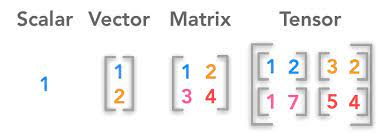
\includegraphics[scale=0.4]{vector}
  \par}
\end{frame}

\begin{frame}[fragile]{Álgebra Lineal Con Python}
  \begin{onlyenv}<1>
      \begin{lstlisting}
    % matplotlib inline
    import matplotlib.pyplot as plt
    plt.imshow(tensor, interpolation='nearest')
    plt.show()
  \end{lstlisting}
\end{onlyenv}

\begin{onlyenv}<2>
  \begin{lstlisting}
tensor = np.array([
		   [[0,0,0,0],  [0,0,0,0], [0,0,0,0]],
		   [[128,128,128], [128,128,128],[128,128,128]],
		   [[255,255,255], [255,255,255], [255,255,255]]
		   ])              

plt.imshow(tensor, interpolation='nearest')
plt.show()
  \end{lstlisting}
               \end{onlyenv}

\end{frame}


\begin{frame}{Repaso de Álgebra Lineal}
  Una embotelladora de refrescos desea cotizar la publicidad de sus productos en televisión,
radio y revista, se tienen tres propuestas del plan de medios de acuerdo con el presupuesto
asignado acerca de la cantidad de anuncios por medio en el transcurso de un mes. En el
primer presupuesto cada anuncio en televisión tiene un coste de \$250 000, en radio \$5 000
y en revista \$30 000. En el segundo presupuesto \$310 000, \$4 000 y \$15 000 y en el último
presupuesto \$560 000, \$10 000 y \$35 000. Los totales por presupuesto son los siguientes:
\$21 795 000, \$31 767 000 y \$61 225 000.
\end{frame}

\begin{frame}{Dimensión de un vector}
  
  \lstinputlisting{scriptsLinAlg/01_dimension_vectors.py}
\end{frame}



\begin{frame}[t]{Transponer, suma de matrices y escalares}
  \begin{onlyenv}<1>
      \lstinputlisting{scriptsLinAlg/02_transpose_sum.py}
    \end{onlyenv}

    \begin{onlyenv}<2>
            \lstinputlisting{scriptsLinAlg/02_sum.py}
    \end{onlyenv}
  \end{frame}

  
%%% Local Variables:
%%% mode: latex
%%% TeX-master: "../slides"
%%% End:

  \section{Matrices}
  
  \begin{frame}[t]{Suma de Matrices (Broadcasting)}
    \lstinputlisting{scriptsLinAlg/03_sum_broadcasting.py}
  \end{frame}


  \begin{frame}{Producto Interno}
    \begin{onlyenv}<1>
      \lstinputlisting{scriptsLinAlg/04_dotproduct.py}    
    \end{onlyenv}

    \only<2>{%
      Suponga que un fabricante produce cuatro artículos. Su demanda está dada por el vector de demanda $\bm{d} =
      \begin{pmatrix}
    30 & 20 & 40 & 10    
      \end{pmatrix}
$ (una matriz de $1 \times 4$). El precio por unidad que recibe el fabricante por los artículos está dado por el vector de precios $\bm{p} =
\begin{pmatrix}
   \$20 \\
   \$15 \\
   \$18 \\
   \$40
\end{pmatrix}
$
(una matriz de $4 \times 1$). Si se cumple la demanda, ¿cuánto dinero recibirá el fabricante?           
}  
  \end{frame}


\label{sec:matrix-operations}

  \begin{frame}{Producto Interno de dos Matrices}{}

    \begin{columns}[t]
      \column{0.5\textwidth }
          Calcular $\bm{AB}$ y $\bm{BA}$. Comentar
    
          \begin{flalign*}
      \bm{A} &= %
      \begin{pmatrix}
         2&  0& -3\\
         4&  1&  5\\
       \end{pmatrix}
       \\[3mm]
      \bm{B} &= %
      \begin{pmatrix}
        7& -1&  4&  7\\
        2&  5&  0& -4\\
        -3&  1&  2&  3\\
      \end{pmatrix}
    \end{flalign*}

    
    
    \column{0.5\textwidth }
    \lstinputlisting[firstline=3]{scriptsLinAlg/05_dotproduct.py}
    \end{columns}


    
  \end{frame}
  
  \begin{frameExample}{Contagios}{}
    \only<1>{%
    En este ejemplo se muestra la forma en la cual se puede usar la multiplicación de matrices para modelar la manera en que se extiende una enfermedad contagiosa. Suponga que cuatro individuos han contraído esta enfermedad. Este grupo entra en contacto con seis personas de
un segundo grupo. Estos contactos, llamados contactos directos, se pueden representar por una matriz de $4 \times 6$. En seguida se da un ejemplo de este tipo de matrices.

\[
  \bm{A} =%
  \begin{pmatrix}
0&1&0&0&1&0\\
1&0&0&1&0&1\\
0&0&0&1&1&0\\
1&0&0&0&0&1\\
\end{pmatrix}
\]
}%

\only<2>{%
  Ahora suponga que un tercer grupo de cinco personas tiene varios contactos directos con individuos del segundo grupo. Esto también se puede representar mediante una matriz. \alert{Matriz de contacto directo}: segundo y tercer grupos. Realizar multiplicación de matrices.

  \[\bm{B} = %
\begin{pmatrix}
  0&0&1&0&1\\
  0&0&0&1&0\\
  0&1&0&0&0\\
  1&0&0&0&1\\
  0&0&0&1&0\\
  0&0&1&0&0\\
\end{pmatrix}
\]

Calcular en número de contactos indirectos entre las personas del grupo 1 y grupo 3.
}



\begin{onlyenv}<3>
  \lstinputlisting[firstline=3]{scriptsLinAlg/05_example-infections.py}
\end{onlyenv}

\end{frameExample}




%%% Local Variables:
%%% mode: latex
%%% TeX-master: "../slides"
%%% End:



\begin{frame}{Propiedades de las matrices}{}
  
  \begin{columns}
    \column{0.7\textwidth}
      \begin{enumerate}[i)] \justifying \parskip3mm
  \item<only@1,2> \alert{Ley asociativa} $A(BC) = (AB)C$ 
  \item<only@1,3> \alert{Ley distributiva} $A(B + C) = AB + AC$ 
  \item<only@1,4> \alert{Ley conmutativa} $AB = BA$ 
  \end{enumerate}
  \column{0.4\textwidth}
  \only<1>{\lstinputlisting[firstline=3,lastline=19]{scriptsLinAlg/06_matrix-properties.py}}
  \only<2>{\lstinputlisting[firstline=21,lastline=23]{scriptsLinAlg/06_matrix-properties.py}}
  \only<3>{\lstinputlisting[firstline=26,lastline=28]{scriptsLinAlg/06_matrix-properties.py}}
  \only<4>{\lstinputlisting[firstline=30,lastline=46]{scriptsLinAlg/06_matrix-properties.py}}
  \end{columns}
\end{frame}

\begin{frame}{Transposición de Producto de Matrices}
  Existe una propiedad que nos dice: \[ (AB)^{T} = B^T A^T \]

  \begin{columns}
    \column{0.5\textwidth}
  \begin{align*}
    \bm{A} & =%
             \begin{pmatrix}
               7&  1\\ 
               2& -3\\ 
               4&  8\\
             \end{pmatrix}
    \\
    \bm{B} &=%
             \begin{pmatrix}
               1& 6 \\
               -2& 3 \\
             \end{pmatrix}
    \\
    \bm{AB}^T &= %
                \begin{pmatrix}
                  5 &  8& -12\\
                  45&   3&  48\\
                \end{pmatrix}
  \end{align*}
  
  \column{0.5\textwidth}
  \begin{align*}
    \bm{B}^T &=%
               \begin{pmatrix}
                 1& -2 \\
                 6& 3 \\
               \end{pmatrix}
    \\
       \bm{A}^T & =%
             \begin{pmatrix}
               7&  2& 4 \\ 
               1& -3& 8 \\ 
             \end{pmatrix}
    \\
    \bm{B}^T\bm{A}^T &= %
                       \begin{pmatrix}
                         1& -2 \\
                         6& 3 \\
                       \end{pmatrix}
    \begin{pmatrix}
      7&  2& 4 \\ 
      1& -3& 8 \\ 
    \end{pmatrix}
  \end{align*}
  \end{columns}
Comprobar con Python
\end{frame}


%%% Local Variables:
%%% mode: latex
%%% TeX-master: "../slides"
%%% End:

\section{Sistemas de Ecuaciones Lineales}
\label{sec:linear-equations}

\begin{frame}{Solución de Un Sistema de Ecuaciones Lineales}

  \begin{columns}
    \column{0.6\textwidth}
      {\centering
  \resizebox{0.9\textwidth}{!}{%
    \begin{tikzpicture}
      
      % Grid
      \draw[black!10,dashed,xstep=1cm] (-6,-6) grid(6,6);
      

      % Axes:
      % Are simply drawn using line with the `->` option to make them arrows:
      % The main labels of the axes can be places using `node`s:
      \draw [->] (-6,0) -- (6,0) node [above left]  {$x$};
      \draw [->] (0,-6) -- (0,6) node [below right] {$y$};

      \draw [name path={blue line}, blue] (-3.94,-6.84) -- (0.79,7.36) node [below right] {$L_1$};
      \draw [name path={red line}, red] (-3.94, -4.894) -- (0.789, 4.57) node [below right] {$L_2$};

      % Intersections
      \fill[name intersections={of=blue line and red line}](intersection-1) circle (3pt);
    \end{tikzpicture}
  }
  \par}

\column{0.3\textwidth}
\begin{onlyenv}<1>
  \begin{align*}
    y &= 3x + 5\\
    y &= 2x + 3\\[5mm]
    3x + 5 & = 2x + 3\\
    3x - 2x &= 3 - 5\\
    x&= \\
    y &= 
  \end{align*}
\end{onlyenv}
\begin{onlyenv}<2>
  \begin{align*}
    y &= 3x + 5\\
    y &= 2x + 3\\[5mm]
    -3x + y &= 5\\
    -2x + y &= 3
  \end{align*}
  \begin{flalign*}
    \bm{A} & =
      \begin{pmatrix}
      -3 & 1\\
      -2 & 1
    \end{pmatrix}
    \\
    \bm{x} &=%
    \begin{pmatrix}
      x \\
      y
    \end{pmatrix}
    \\
    \bm{b} &=%
    \begin{pmatrix}
      5 \\
      3
    \end{pmatrix}
  \end{flalign*}
\end{onlyenv}
  \end{columns}
\end{frame}

\begin{frame}{Tipos Especiales de Matrices}
  \begin{columns}
    \column{0.4\textwidth}
      \begin{itemize} \justifying \parskip3mm
  \item Matriz Identidad $I$.
  \item  Matriz Inversa $A^{-1}$.
  \item  Matriz Singular.
  \end{itemize}
  \column{0.6\textwidth}
  \lstinputlisting[firstline=3]{scriptsLinAlg/09_special-matrix.py}
  \end{columns}
\end{frame}

\begin{frame}{Solución de Ecuaciones con Matriz Inversa}

  \begin{theorem}\justifying
    Si $\bm{A}$ es una matriz  invertible de $n \times n$, entonces para toda matriz $\bm{b}$ de $n \times 1$, el sistema de ecuaciones $A\bm{x} = \bm{b}$ tiene exactamente una solucioń; a saber, $\bm{x} = A^{-1}\bm{b}$
  \end{theorem}
  \begin{flalign*}
    x_1 + x_2 + 2x_3 & = 9\\
    2x_1 + 4x_2 - 3x_3 & = 1\\
    3x_1 + 6x_2 - 5x_3 & = 0\\
  \end{flalign*}
\end{frame}




\begin{frame}{Sistemas Sin Solución, Una Solución, Infinitas Soluciones}

  Todo sistema de Ecuaciones lineales no tiene soluciones, tiene exactamente una solución o tiene una infinidad de soluciones.

  \begin{columns}[t]
    \column{0.3\textwidth}
      \begin{flalign*} 
  y &= 3x + 5 \\
  y &= 6x  + 7 \\
  y &= \frac{5}{2}x - 1  
\end{flalign*}

\column{0.3\textwidth}
\begin{flalign*}
  y &= \nicefrac{1}{2}x + 0.5 \\
  y &= \nicefrac{-3}{5}x + \nicefrac{8}{5}\\
  y &= \nicefrac{-4}{3}x + \nicefrac{7}{3} 
\end{flalign*}
\column{0.3\textwidth}
\begin{flalign*}
  y &= 2x + 5 \\
  y &= 2x + 5
\end{flalign*}
  \end{columns}
  
\end{frame}


\begin{frame}{Graficar Vectores}
  \begin{block}{Definición algebraica de un vector} \justifying
     Un \alert{vector $\bm{v}$} en el plano $xy$ es un par ordenado de números reales $(a, b)$. Los
números $a$ y $b$ se denominan \alert{elementos} o \alert{componentes} del vector $\bm{v}$. El \alert{vector cero} es el vector $(0, 0)$.
\end{block}

\lstinputlisting[firstline=10, lastline=23]{scriptsLinAlg/11_plot-vectors.py}
\end{frame}

\begin{frame}{Combinaciones Lineales}
  \begin{block}<only@1>{Combinación Lineal} \justifying
    Sean $\bm{v}_1, \bm{v}_2, \ldots, \bm{v}_n$ vectores en un espacio vectorial $V$. Entonces cualquier vector de la forma \[a_1v_1+ a_2v_2+ \cdots+ a_nv_n \] donde, $a_1, a_2, \ldots, a_n$ son escalares se denomina una \alert{combinación lineal} de $\bm{v}_1, \bm{v}_2, \ldots, \bm{v}_n$
  \end{block}

  \begin{onlyenv}<2>
      \begin{columns}[t]
    \column{0.5\textwidth}
    \lstinputlisting[firstline=3,lastline=14]{scriptsLinAlg/12_linear-combinations.py}
    \column{0.4\textwidth}
    \lstinputlisting[firstline=16]{scriptsLinAlg/12_linear-combinations.py}
  \end{columns}
  \end{onlyenv}
\end{frame}


\begin{frame}{Espacios y Subespacios}
  Los conjuntos $\mathbb{R}^2$ y $\mathbb{R}^3$ junto con las operaciones de suma de vectores y multiplicación por un escalar se denominan \alert{espacios vectoriales}. Se puede decir, de forma intuitiva, que un espacio vectorial es un conjunto de objetos con dos operaciones que obedecen las reglas que acaban de escribirse.
\end{frame}


\begin{frame}{Independencia Lineal}
  

      Sean $\bm{v}_1 , \bm{v}_2 , \ldots , \bm{v}_n$ , $n$ vectores en un espacio vectorial $V$. Entonces se dice que los vectores son \alert{linealmente dependientes} si existen $n$ escalares $c_1 , c_2 ,\ldots, c_n$ \emph{no todos cero} tales que $c_1 \bm{v}_1 + c_2 \bm{v}_2 + \cdots + c_n\bm{v}_n = \bm{0}$.  Si los vectores no son linealmente dependientes, se dice que son \alert{linealmente independientes}.


    ¿Existe alguna relación especial entre los vectores $\bm{v}_1 =
    \begin{pmatrix}
      1\\
      2\\
    \end{pmatrix}
$ y $\bm{v}_2 =
    \begin{pmatrix}
      2\\
      4\\
    \end{pmatrix}$? ¿Qué tienen de especial los vectores $\bm{v}_1 =
    \begin{pmatrix}
      1\\
      2\\
      3\\
    \end{pmatrix}
$, $\bm{v}_2 =
    \begin{pmatrix}
      -4\\
      1\\
5\\
    \end{pmatrix}$ y $\bm{v}_3 =
    \begin{pmatrix}
      -5\\
      8\\
19
    \end{pmatrix}$?
\end{frame}

\begin{frame}{¿Existe la Inversa de Una Matriz?}
\only<1>{%
  Una matriz es singular si tiene un vector linealmente dependiente en sus filas o columnas. Si removemos el vector linealmente independiente de la matriz, la matriz deja de ser cuadrada.
  
  \lstinputlisting[firstline=3]{scriptsLinAlg/15_singular.py}
}

\begin{block}<only@2>{ Valor característico y vector característico}\justifying
  Sea $A$ una matriz de $n \times n$ con componentes reales. El número $\lambda$ (real o complejo) se denomina \alert{valor característico} de $A$ si existe un vector diferente de cero $\bm{v}$ en $\mathbb{C}^n$ tal que \[\bm{Av} = \bm{\lambda v} \]

  El vector $\bm{v} \neq \bm{0}$ se denomina \alert{vector característico} de $A$ correspondiente al \alert{valor característico} de $\lambda$
\end{block}

\begin{exampleblock}<only@3>{Ejemplo}\justifying
  Sea $A =
  \begin{pmatrix}
    10 & -18 \\
    6 & -11 \\
  \end{pmatrix}
$. Entonces $A
\begin{pmatrix}
  2\\
  1\\
\end{pmatrix}
=
\begin{pmatrix}
    10 & -18 \\
    6 & -11 \\
  \end{pmatrix}
  \begin{pmatrix}
  2\\
  1\\
\end{pmatrix}
=
  \begin{pmatrix}
  2\\
  1\\
\end{pmatrix}
$. Así, $\lambda = 1$ es un valor característico de $A$ con el correspondiente vector característico $\bm{v_1} =
\begin{pmatrix}
  2\\
  1
\end{pmatrix}
$
\end{exampleblock}
\begin{exampleblock}<only@4>{Otro ejemplo de Vectores y Valores Propios} \justifying
  $A
\begin{pmatrix}
  3\\
  2\\
\end{pmatrix}
=
\begin{pmatrix}
    10 & -18 \\
    6 & -11 \\
  \end{pmatrix}
  \begin{pmatrix}
  3\\
  2\\
\end{pmatrix}
=
  \begin{pmatrix}
  -6\\
  -4
\end{pmatrix}
= -2
  \begin{pmatrix}
  3\\
  2
\end{pmatrix}
$, de modo que $\lambda_2 = -2$ es un valor característico (propio) de $A$ con el correspondiente vector característico (propio) $\bm{v}_2 =
\begin{pmatrix}
  3\\
  2
\end{pmatrix}
$.
\end{exampleblock}
\end{frame}


%%% Local Variables:
%%% mode: latex
%%% TeX-master: "../slides"
%%% End:


\section{Operaciones Básicas}
\label{sec:basic-operations}

\begin{frame}[fragile]{Repaso de Álgebra Lineal}
  \begin{columns}[t]
    \column{0.2\textwidth}
    \begin{itemize} \justifying \parskip3mm
  \item<only@1-3> Escalar
  \item<only@1-3> Vector
  \item<only@1-4> Matriz
  \item<only@1-4> Tensor
  \end{itemize}

  \column{0.8\textwidth}
  {\centering
    \includegraphics<1>[scale=0.4]{scalar-vector-matrix}
    \includegraphics<1>[scale=0.5]{tensor_shape}
    
    \includegraphics<1>[scale=0.5]{tensor}
    \par}

  \begin{onlyenv}<2>
    \begin{ipythonnb}[1]
import numpy as np
    \end{ipythonnb}
    
    \begin{ipythonnb}
x = np.array(12)
x.ndim
    \end{ipythonnb}
    \begin{ipythonnb2}
0
    \end{ipythonnb2}
\end{onlyenv}

  \begin{onlyenv}<3>
      \begin{ipythonnb}
x = np.array([12, 3, 6, 14, 7])
x
\end{ipythonnb}

\begin{ipythonnb2}
array([12,3,6,14,7])
\end{ipythonnb2}

\begin{ipythonnb}
x.ndim
\end{ipythonnb}

\begin{ipythonnb2}
  1
\end{ipythonnb2}

\end{onlyenv}

  \begin{onlyenv}<4>
    \begin{ipythonnb}
x = np.array([[5, 78, 2, 34, 0],
              [6, 79, 3, 35, 1],
              [7, 80, 4, 36, 2]])

x.ndim
\end{ipythonnb}

      \begin{ipythonnb}
        tensor = np.array([
        [[5, 78, 2, 34, 0],
         [6, 79, 3, 35, 1],
         [7, 80, 4, 36, 2]],
        [[5, 78, 2, 34, 0],
         [6, 79, 3, 35, 1],
         [7, 80, 4, 36, 2]],
        [[5, 78, 2, 34, 0],
         [6, 79, 3, 35, 1],
         [7, 80, 4, 36, 2]]
        ])
\end{ipythonnb}
\end{onlyenv}

  \end{columns}
\end{frame}



\begin{frame}[fragile]{Álgebra Lineal Con Python}
  \begin{onlyenv}<1>
      \begin{lstlisting}
    % matplotlib inline
    import matplotlib.pyplot as plt
    plt.imshow(tensor, interpolation='nearest')
    plt.show()
  \end{lstlisting}
\end{onlyenv}

\begin{onlyenv}<2>
  \begin{lstlisting}
tensor = np.array([
		   [[0,0,0,0],  [0,0,0,0], [0,0,0,0]],
		   [[128,128,128], [128,128,128],[128,128,128]],
		   [[255,255,255], [255,255,255], [255,255,255]]
		   ])              

plt.imshow(tensor, interpolation='nearest')
plt.show()
  \end{lstlisting}
               \end{onlyenv}

\end{frame}


\begin{frame}{Repaso de Álgebra Lineal}
  Una embotelladora de refrescos desea cotizar la publicidad de sus productos en televisión,
radio y revista, se tienen tres propuestas del plan de medios de acuerdo con el presupuesto
asignado acerca de la cantidad de anuncios por medio en el transcurso de un mes. En el
primer presupuesto cada anuncio en televisión tiene un coste de \$250 000, en radio \$5 000
y en revista \$30 000. En el segundo presupuesto \$310 000, \$4 000 y \$15 000 y en el último
presupuesto \$560 000, \$10 000 y \$35 000. Los totales por presupuesto son los siguientes:
\$21 795 000, \$31 767 000 y \$61 225 000.
\end{frame}

\begin{frame}{Dimensión de un vector}
  
  \lstinputlisting{scriptsLinAlg/01_dimension_vectors.py}
\end{frame}



\begin{frame}[t]{Transponer, suma de matrices y escalares}
  \begin{onlyenv}<1>
      \lstinputlisting{scriptsLinAlg/02_transpose_sum.py}
    \end{onlyenv}

    \begin{onlyenv}<2>
            \lstinputlisting{scriptsLinAlg/02_sum.py}
    \end{onlyenv}
  \end{frame}


  \section{Matrices}
  
  \begin{frame}[t]{Suma de Matrices (Broadcasting)}
    \lstinputlisting{scriptsLinAlg/03_sum_broadcasting.py}
  \end{frame}


  \begin{frame}{Producto Interno}
    \begin{onlyenv}<1>
      \lstinputlisting{scriptsLinAlg/04_dotproduct.py}    
    \end{onlyenv}

    \only<2>{%
      Suponga que un fabricante produce cuatro artículos. Su demanda está dada por el vector de demanda $\bm{d} =
      \begin{pmatrix}
    30 & 20 & 40 & 10    
      \end{pmatrix}
$ (una matriz de $1 \times 4$). El precio por unidad que recibe el fabricante por los artículos está dado por el vector de precios $\bm{p} =
\begin{pmatrix}
   \$20 \\
   \$15 \\
   \$18 \\
   \$40
\end{pmatrix}
$
(una matriz de $4 \times 1$). Si se cumple la demanda, ¿cuánto dinero recibirá el fabricante?           
}  
  \end{frame}


\label{sec:matrix-operations}

  \begin{frame}{Producto Interno de dos Matrices}{}

    \begin{columns}[t]
      \column{0.5\textwidth }
          Calcular $\bm{AB}$ y $\bm{BA}$. Comentar
    
          \begin{flalign*}
      \bm{A} &= %
      \begin{pmatrix}
         2&  0& -3\\
         4&  1&  5\\
       \end{pmatrix}
       \\[3mm]
      \bm{B} &= %
      \begin{pmatrix}
        7& -1&  4&  7\\
        2&  5&  0& -4\\
        -3&  1&  2&  3\\
      \end{pmatrix}
    \end{flalign*}

    
    
    \column{0.5\textwidth }
    \lstinputlisting[firstline=3]{scriptsLinAlg/05_dotproduct.py}
    \end{columns}


    
  \end{frame}
  
  \begin{frameExample}{Contagios}{}
    \only<1>{%
    En este ejemplo se muestra la forma en la cual se puede usar la multiplicación de matrices para modelar la manera en que se extiende una enfermedad contagiosa. Suponga que cuatro individuos han contraído esta enfermedad. Este grupo entra en contacto con seis personas de
un segundo grupo. Estos contactos, llamados contactos directos, se pueden representar por una matriz de $4 \times 6$. En seguida se da un ejemplo de este tipo de matrices.

\[
  \bm{A} =%
  \begin{pmatrix}
0&1&0&0&1&0\\
1&0&0&1&0&1\\
0&0&0&1&1&0\\
1&0&0&0&0&1\\
\end{pmatrix}
\]
}%

\only<2>{%
  Ahora suponga que un tercer grupo de cinco personas tiene varios contactos directos con individuos del segundo grupo. Esto también se puede representar mediante una matriz. \alert{Matriz de contacto directo}: segundo y tercer grupos. Realizar multiplicación de matrices.

  \[\bm{B} = %
\begin{pmatrix}
  0&0&1&0&1\\
  0&0&0&1&0\\
  0&1&0&0&0\\
  1&0&0&0&1\\
  0&0&0&1&0\\
  0&0&1&0&0\\
\end{pmatrix}
\]

Calcular en número de contactos indirectos entre las personas del grupo 1 y grupo 3.
}



\begin{onlyenv}<3>
  \lstinputlisting[firstline=3]{scriptsLinAlg/05_example-infections.py}
\end{onlyenv}

\end{frameExample}




%%% Local Variables:
%%% mode: latex
%%% TeX-master: "../slides"
%%% End:



\begin{frame}{Propiedades de las matrices}{}
  
  \begin{columns}
    \column{0.7\textwidth}
      \begin{enumerate}[i)] \justifying \parskip3mm
  \item<only@1,2> \alert{Ley asociativa} $A(BC) = (AB)C$ 
  \item<only@1,3> \alert{Ley distributiva} $A(B + C) = AB + AC$ 
  \item<only@1,4> \alert{Ley conmutativa} $AB = BA$ 
  \end{enumerate}
  \column{0.4\textwidth}
  \only<1>{\lstinputlisting[firstline=3,lastline=19]{scriptsLinAlg/06_matrix-properties.py}}
  \only<2>{\lstinputlisting[firstline=21,lastline=23]{scriptsLinAlg/06_matrix-properties.py}}
  \only<3>{\lstinputlisting[firstline=26,lastline=28]{scriptsLinAlg/06_matrix-properties.py}}
  \only<4>{\lstinputlisting[firstline=30,lastline=46]{scriptsLinAlg/06_matrix-properties.py}}
  \end{columns}
\end{frame}

\begin{frame}{Transposición de Producto de Matrices}
  Existe una propiedad que nos dice: \[ (AB)^{T} = B^T A^T \]

  \begin{columns}
    \column{0.5\textwidth}
  \begin{align*}
    \bm{A} & =%
             \begin{pmatrix}
               7&  1\\ 
               2& -3\\ 
               4&  8\\
             \end{pmatrix}
    \\
    \bm{B} &=%
             \begin{pmatrix}
               1& 6 \\
               -2& 3 \\
             \end{pmatrix}
    \\
    \bm{AB}^T &= %
                \begin{pmatrix}
                  5 &  8& -12\\
                  45&   3&  48\\
                \end{pmatrix}
  \end{align*}
  
  \column{0.5\textwidth}
  \begin{align*}
    \bm{B}^T &=%
               \begin{pmatrix}
                 1& -2 \\
                 6& 3 \\
               \end{pmatrix}
    \\
       \bm{A}^T & =%
             \begin{pmatrix}
               7&  2& 4 \\ 
               1& -3& 8 \\ 
             \end{pmatrix}
    \\
    \bm{B}^T\bm{A}^T &= %
                       \begin{pmatrix}
                         1& -2 \\
                         6& 3 \\
                       \end{pmatrix}
    \begin{pmatrix}
      7&  2& 4 \\ 
      1& -3& 8 \\ 
    \end{pmatrix}
  \end{align*}
  \end{columns}
Comprobar con Python
\end{frame}


\begin{frame}{Solución de Un Sistema de Ecuaciones Lineales}

  \begin{columns}
    \column{0.6\textwidth}
      {\centering
  \resizebox{0.9\textwidth}{!}{%
    \begin{tikzpicture}
      
      % Grid
      \draw[black!10,dashed,xstep=1cm] (-6,-6) grid(6,6);
      

      % Axes:
      % Are simply drawn using line with the `->` option to make them arrows:
      % The main labels of the axes can be places using `node`s:
      \draw [->] (-6,0) -- (6,0) node [above left]  {$x$};
      \draw [->] (0,-6) -- (0,6) node [below right] {$y$};

      \draw [name path={blue line}, blue] (-3.94,-6.84) -- (0.79,7.36) node [below right] {$L_1$};
      \draw [name path={red line}, red] (-3.94, -4.894) -- (0.789, 4.57) node [below right] {$L_2$};

      % Intersections
      \fill[name intersections={of=blue line and red line}](intersection-1) circle (3pt);
    \end{tikzpicture}
  }
  \par}

\column{0.3\textwidth}
\begin{onlyenv}<1>
  \begin{align*}
    y &= 3x + 5\\
    y &= 2x + 3\\[5mm]
    3x + 5 & = 2x + 3\\
    3x - 2x &= 3 - 5\\
    x&= \\
    y &= 
  \end{align*}
\end{onlyenv}
\begin{onlyenv}<2>
  \begin{align*}
    y &= 3x + 5\\
    y &= 2x + 3\\[5mm]
    -3x + y &= 5\\
    -2x + y &= 3
  \end{align*}
  \begin{flalign*}
    \bm{A} & =
      \begin{pmatrix}
      -3 & 1\\
      -2 & 1
    \end{pmatrix}
    \\
    \bm{x} &=%
    \begin{pmatrix}
      x \\
      y
    \end{pmatrix}
    \\
    \bm{b} &=%
    \begin{pmatrix}
      5 \\
      3
    \end{pmatrix}
  \end{flalign*}
\end{onlyenv}
  \end{columns}
\end{frame}

\begin{frame}{Tipos Especiales de Matrices}
  \begin{columns}
    \column{0.4\textwidth}
      \begin{itemize} \justifying \parskip3mm
  \item Matriz Identidad $I$.
  \item  Matriz Inversa $A^{-1}$.
  \item  Matriz Singular.
  \end{itemize}
  \column{0.6\textwidth}
  \lstinputlisting[firstline=3]{scriptsLinAlg/09_special-matrix.py}
  \end{columns}
\end{frame}

\begin{frame}{Solución de Ecuaciones con Matriz Inversa}

  \begin{theorem}\justifying
    Si $\bm{A}$ es una matriz  invertible de $n \times n$, entonces para toda matriz $\bm{b}$ de $n \times 1$, el sistema de ecuaciones $A\bm{x} = \bm{b}$ tiene exactamente una solucioń; a saber, $\bm{x} = A^{-1}\bm{b}$
  \end{theorem}
  \begin{flalign*}
    x_1 + x_2 + 2x_3 & = 9\\
    2x_1 + 4x_2 - 3x_3 & = 1\\
    3x_1 + 6x_2 - 5x_3 & = 0\\
  \end{flalign*}
\end{frame}


\section{Sistemas de Ecuaciones Lineales}
\label{sec:linear-equations}

\begin{frame}{Sistemas Sin Solución, Una Solución, Infinitas Soluciones}

  Todo sistema de Ecuaciones lineales no tiene soluciones, tiene exactamente una solución o tiene una infinidad de soluciones.

  \begin{columns}[t]
    \column{0.3\textwidth}
      \begin{flalign*} 
  y &= 3x + 5 \\
  y &= 6x  + 7 \\
  y &= \frac{5}{2}x - 1  
\end{flalign*}

\column{0.3\textwidth}
\begin{flalign*}
  y &= \nicefrac{1}{2}x + 0.5 \\
  y &= \nicefrac{-3}{5}x + \nicefrac{8}{5}\\
  y &= \nicefrac{-4}{3}x + \nicefrac{7}{3} 
\end{flalign*}
\column{0.3\textwidth}
\begin{flalign*}
  y &= 2x + 5 \\
  y &= 2x + 5
\end{flalign*}
  \end{columns}
  
\end{frame}


\begin{frame}{Graficar Vectores}
  \begin{block}{Definición algebraica de un vector} \justifying
     Un \alert{vector $\bm{v}$} en el plano $xy$ es un par ordenado de números reales $(a, b)$. Los
números $a$ y $b$ se denominan \alert{elementos} o \alert{componentes} del vector $\bm{v}$. El \alert{vector cero} es el vector $(0, 0)$.
\end{block}

\lstinputlisting[firstline=10, lastline=23]{scriptsLinAlg/11_plot-vectors.py}
\end{frame}

\begin{frame}{Combinaciones Lineales}
  \begin{block}<only@1>{Combinación Lineal} \justifying
    Sean $\bm{v}_1, \bm{v}_2, \ldots, \bm{v}_n$ vectores en un espacio vectorial $V$. Entonces cualquier vector de la forma \[a_1v_1+ a_2v_2+ \cdots+ a_nv_n \] donde, $a_1, a_2, \ldots, a_n$ son escalares se denomina una \alert{combinación lineal} de $\bm{v}_1, \bm{v}_2, \ldots, \bm{v}_n$
  \end{block}

  \begin{onlyenv}<2>
      \begin{columns}[t]
    \column{0.5\textwidth}
    \lstinputlisting[firstline=3,lastline=14]{scriptsLinAlg/12_linear-combinations.py}
    \column{0.4\textwidth}
    \lstinputlisting[firstline=16]{scriptsLinAlg/12_linear-combinations.py}
  \end{columns}
  \end{onlyenv}
\end{frame}


\begin{frame}{Espacios y Subespacios}
  Los conjuntos $\mathbb{R}^2$ y $\mathbb{R}^3$ junto con las operaciones de suma de vectores y multiplicación por un escalar se denominan \alert{espacios vectoriales}. Se puede decir, de forma intuitiva, que un espacio vectorial es un conjunto de objetos con dos operaciones que obedecen las reglas que acaban de escribirse.
\end{frame}


\begin{frame}{Independencia Lineal}
  

      Sean $\bm{v}_1 , \bm{v}_2 , \ldots , \bm{v}_n$ , $n$ vectores en un espacio vectorial $V$. Entonces se dice que los vectores son \alert{linealmente dependientes} si existen $n$ escalares $c_1 , c_2 ,\ldots, c_n$ \emph{no todos cero} tales que $c_1 \bm{v}_1 + c_2 \bm{v}_2 + \cdots + c_n\bm{v}_n = \bm{0}$.  Si los vectores no son linealmente dependientes, se dice que son \alert{linealmente independientes}.


    ¿Existe alguna relación especial entre los vectores $\bm{v}_1 =
    \begin{pmatrix}
      1\\
      2\\
    \end{pmatrix}
$ y $\bm{v}_2 =
    \begin{pmatrix}
      2\\
      4\\
    \end{pmatrix}$? ¿Qué tienen de especial los vectores $\bm{v}_1 =
    \begin{pmatrix}
      1\\
      2\\
      3\\
    \end{pmatrix}
$, $\bm{v}_2 =
    \begin{pmatrix}
      -4\\
      1\\
5\\
    \end{pmatrix}$ y $\bm{v}_3 =
    \begin{pmatrix}
      -5\\
      8\\
19
    \end{pmatrix}$?
\end{frame}

\begin{frame}{¿Existe la Inversa de Una Matriz?}
\only<1>{%
  Una matriz es singular si tiene un vector linealmente dependiente en sus filas o columnas. Si removemos el vector linealmente independiente de la matriz, la matriz deja de ser cuadrada.
  
  \lstinputlisting[firstline=3]{scriptsLinAlg/15_singular.py}
}

\begin{block}<only@2>{ Valor característico y vector característico}\justifying
  Sea $A$ una matriz de $n \times n$ con componentes reales. El número $\lambda$ (real o complejo) se denomina \alert{valor característico} de $A$ si existe un vector diferente de cero $\bm{v}$ en $\mathbb{C}^n$ tal que \[\bm{Av} = \bm{\lambda v} \]

  El vector $\bm{v} \neq \bm{0}$ se denomina \alert{vector característico} de $A$ correspondiente al \alert{valor característico} de $\lambda$
\end{block}

\begin{exampleblock}<only@3>{Ejemplo}\justifying
  Sea $A =
  \begin{pmatrix}
    10 & -18 \\
    6 & -11 \\
  \end{pmatrix}
$. Entonces $A
\begin{pmatrix}
  2\\
  1\\
\end{pmatrix}
=
\begin{pmatrix}
    10 & -18 \\
    6 & -11 \\
  \end{pmatrix}
  \begin{pmatrix}
  2\\
  1\\
\end{pmatrix}
=
  \begin{pmatrix}
  2\\
  1\\
\end{pmatrix}
$. Así, $\lambda = 1$ es un valor característico de $A$ con el correspondiente vector característico $\bm{v_1} =
\begin{pmatrix}
  2\\
  1
\end{pmatrix}
$
\end{exampleblock}
\begin{exampleblock}<only@4>{Otro ejemplo de Vectores y Valores Propios} \justifying
  $A
\begin{pmatrix}
  3\\
  2\\
\end{pmatrix}
=
\begin{pmatrix}
    10 & -18 \\
    6 & -11 \\
  \end{pmatrix}
  \begin{pmatrix}
  3\\
  2\\
\end{pmatrix}
=
  \begin{pmatrix}
  -6\\
  -4
\end{pmatrix}
= -2
  \begin{pmatrix}
  3\\
  2
\end{pmatrix}
$, de modo que $\lambda_2 = -2$ es un valor característico (propio) de $A$ con el correspondiente vector característico (propio) $\bm{v}_2 =
\begin{pmatrix}
  3\\
  2
\end{pmatrix}
$.
\end{exampleblock}
\end{frame}


 
\section{Normas}
\label{sec:norms}

\begin{frame}{Uso de la Norma}
  ¿Cómo medimos el tamaño de un vector?. \href{https://en.wikipedia.org/wiki/Norm_(mathematics)}{Definición De Norma aquí}

  \begin{columns}[t]
    \column{0.5\textwidth}
  \lstinputlisting[firstline=3, lastline=18]{scriptsLinAlg/16_norms.py}
  \column{0.5\textwidth}
    \lstinputlisting[firstline=19]{scriptsLinAlg/16_norms.py}
  \end{columns}

\end{frame}


\begin{frame}{Tipos de Norma}
    \lstinputlisting[firstline=3]{scriptsLinAlg/17_norm-types.py}
\end{frame}

\begin{frame}{Producto Interno Con Normas}
  \lstinputlisting[firstline=3]{scriptsLinAlg/18_norms_dot-product.py}
\end{frame}

\section{Matrices Especiales}
\label{sec:special-matrices}


\begin{frame}{La matriz diagonal y la matriz simétrica}
\lstinputlisting[firstline=3]{scriptsLinAlg/19_diagonal-symmetric.py}
\end{frame}

\begin{frame}{Vectores ortogonales y  Matrices Ortogonales}
  
  \begin{block}<only@1>{Matriz Ortogonal}\justifying
    Una matriz de $Q$ de $n\times n$ se llama \alert{ortogonal} si $Q$ es invertible y \[Q^{-1} = Q^{T} \]. Observe que si $Q^{-1} = Q^{T}$, entonces $Q^TQ = I$
  \end{block}

  \begin{onlyenv}<2>
    \begin{columns}[t]
      \column{0.5\textwidth}
      \lstinputlisting[firstline=3,lastline=23]{scriptsLinAlg/20_orthogonal.py}
      \column{0.5\textwidth}
      \lstinputlisting[firstline=25]{scriptsLinAlg/20_orthogonal.py}
    \end{columns}
  \end{onlyenv}
    \begin{onlyenv}<3>
    \begin{columns}[t]
      \column{0.5\textwidth}
      \lstinputlisting[firstline=3,lastline=19]{scriptsLinAlg/21_orthonormal.py}
      \column{0.5\textwidth}
      \lstinputlisting[firstline=21]{scriptsLinAlg/21_orthonormal.py}
    \end{columns}
  \end{onlyenv}

\end{frame}

\begin{frame}{Determinante y Traza}
  \only<1>{\lstinputlisting[firstline=3]{scriptsLinAlg/22_trace.py}}
  \only<2>{\lstinputlisting[firstline=3]{scriptsLinAlg/23_determinant.py}}
\end{frame}

%%% Local Variables:
%%% mode: latex
%%% TeX-master: "../slides"
%%% End:


% ==============================
\begin{frame}
  \maketitle
\end{frame}


\end{document}
